\documentclass[xcolor=dvipsnames]{beamer}
%\documentclass[xcolor=dvipsnames]{article}
%\usepackage{beamerarticle}
\usepackage[english]{babel}
\usepackage[T1]{fontenc}
\usepackage[utf8]{inputenc}
%\usepackage{cmbright}
%\usepackage[default]{gfsneohellenic}
%\usepackage{gfsartemisia-euler}
%\usepackage[sfdefault]{cabin}
%\usepackage[default]{comfortaa} % good one, rounded letters
%\usepackage[default]{lato}
\usepackage[math]{kurier} % good one, letters with several componetns
%\usepackage[math]{anttor}
\usepackage{yfonts}

\hypersetup{
  colorlinks=true,
  citecolor=brown!70!black,
  linkcolor=brown!80!black,
  urlcolor=blue!70!black,
}

\definecolor{linkcol}{rgb}{0,0,0.4} 
\definecolor{citecol}{rgb}{0.5,0,0} 
\definecolor{darkblue}{rgb}{.0,.0,.6}
\definecolor{darkgreen}{rgb}{.0,.4,.0}
\definecolor{darkred}{rgb}{.8,.0,.0}



\usepackage{graphicx}
\usepackage{color, subfigure, wrapfig, afterpage,
  fancyhdr, graphicx, calc, url, 
  boxedminipage, xspace, lscape, stfloats, 
  todonotes, amsmath,amsthm, amssymb, mathtools, etoolbox,
  tikz, tikz-cd, ifsym, colortbl}
\usepackage[mathscr]{euscript}

\usetikzlibrary{shapes, calc, fadings,
                arrows, automata, positioning,
                decorations.markings, arrows.meta}

\PassOptionsToPackage{hyphens}{url}\usepackage{hyperref}

\DeclareMathAlphabet{\mathpzc}{OT1}{pzc}{m}{it}


\newcommand{\rX}{\langle X \rangle}
\newcommand{\rY}{\langle Y \rangle}

\newcommand{\tracetree}{{\tt tracetree}}
\newcommand{\Tracetree}{{\tt Tracetree}}
\newcommand{\traceroute}{{\tt traceroute}}
\newcommand{\wdata}{{\tt woolthorpe} dataset}
\newcommand{\ovhdata}{{\tt ovh} dataset}
\newcommand{\ip}{{\sc ip}}
\newcommand{\erdosrenyi}{Erdős–Rényi }
\newcommand{\ok}{\scalebox{2}{\color{mycolor} \ensuremath \checkmark}}

\newcommand{\lapente}{\alpha}



\DeclareMathOperator{\p}{P}
\DeclareMathOperator{\round}{round}
\DeclareMathOperator{\Var}{Var}
\DeclareMathOperator{\Ob}{Ob}
\DeclareMathOperator{\Pois}{Pois}
\DeclareMathOperator{\mor}{or }
\DeclareMathOperator{\Perror}{P_{error}}
\DeclareMathOperator{\links}{Links}
\DeclareMathOperator{\nodes}{Nodes}
\DeclareMathOperator{\spath}{Sp}
\DeclareMathOperator{\newspath}{path_{new}}
\DeclareMathOperator{\pchange}{\mathit {P_{change}}}


%\newcommand{\sps}{\mathit{sps}}
\newcommand{\sps}{S}
\newcommand{\varsps}{S}
\newcommand{\SPS}{\mathit{SPS}}
\newcommand{\spt}{\mathit{spt}}

\DeclareMathAlphabet{\mathpzc}{OT1}{pzc}{m}{it}
\newcommand{\D}{\mathpzc{d}}
\newcommand{\E}{\mathbb{E}}
\newcommand{\N}{\mathbb{N}}
\newcommand{\R}{\mathbb{R}}
\newcommand{\disttilde}[1]{
  \stackrel{\scriptscriptstyle #1}{\widetilde{uv}}}
\newcommand{\prodisttilde}[3]{
  \stackrel{\scriptscriptstyle #1}{\widetilde {#2#3}}}

\newcommand{\dist}{\text{dist=}}
\newcommand{\col}{\text{color}}
\newcommand{\diam}{\text{diam}}
\newcommand{\boldall}{\boldmath\bf}
\newcommand{\orG}{\overrightarrow{G}}
\newcommand{\lmapsto}{\xmapsto{\hspace{1em}}}

\newcommand{\prodist}[3]{
  \stackrel{\scriptscriptstyle #1}{\widetilde {#2#3}}}

\newenvironment{blockquote}{%
  \par%
  \medskip
  \leftskip=1.5em\rightskip=2em%
  \noindent\ignorespaces}{%
  \par\medskip}


\everymath{\displaystyle}

%%%%%%%%%%%%%%%%%%%%%%%%%%%%%%%%%%%%%%%%%%%%%%%%%%%%%%%%%%%%%%%%%
% some commands

\newcommand{\donc}{\ensuremath\Longrightarrow\,}

\newcommand{\deuxminpg}[4]{
  \begin{minipage}{#2}
    #1
  \end{minipage}
  \begin{minipage}{#4}
    #3
  \end{minipage}
}

\newcommand{\deuxminpgt}[4]{
  \begin{minipage}[t]{#2}
    #1
  \end{minipage}
  \begin{minipage}[t]{#4}
    #3
  \end{minipage}
}

\newcommand{\troisminpg}[6]{
\begin{minipage}{#2}
#1
\end{minipage}
\begin{minipage}{#4}
#3
\end{minipage}
\begin{minipage}{#6}
#5
\end{minipage}
}

\newcommand{\troisminpgt}[6]{
\begin{minipage}[b]{#2}
#1
\end{minipage}
\begin{minipage}{#4}
#3
\end{minipage}
\begin{minipage}{#6}
#5
\end{minipage}
}

\def\Put(#1,#2)#3{\leavevmode\makebox(0,0){\put(#1,#2){#3}}}

% end of some commands
%%%%%%%%%%%%%%%%%%%%%%%%%%%%%%%%%%%%%%%%%%%%%%%%%%%%%%%%%%%%%%%%%%


%%%%%%%%%%%%%%%%% beamer configuration %%%%%%%%%%%%%%%%%%%%%%%%%%
%%%%%%%%%%%%%%%%%%%%%%%%%%%%%%%%%%%%%%%%%%%%%%%%%%%%%%%%%%%%%%%%%

\definecolor{mycolor}{HTML}{484BBA}
\definecolor{mycolor2}{HTML}{73A0C5}
\usecolortheme[named=black]{structure}

\definecolor{MYblue}{HTML}{73A0C5}
\definecolor{MYlightbrown}{HTML}{D2965A}
\definecolor{MYdarkblue}{HTML}{072e39}
\definecolor{MYdarkbrown}{HTML}{86592C}
\definecolor{MYlightblue}{HTML}{2C7186}
\definecolor{MYgreen}{HTML}{5AA866}
\definecolor{MYred}{HTML}{FF4748}
%\usetheme{Rochester}
%\usecolortheme{structure}
\useinnertheme{rectangles}

\definecolor{AA}{HTML}{572762}
\definecolor{A}{HTML}{1A5882}
\definecolor{B}{HTML}{713657}
\definecolor{C}{HTML}{0C8F7F}
\definecolor{D}{HTML}{914747}
\definecolor{E}{HTML}{446E8F}
\definecolor{F}{HTML}{10633D}

%% blue on white toc
%% \setbeamercolor{section in toc}{fg=mycolor2!40!black}
%% \setbeamercolor{subsection in toc}{fg=mycolor2!60!black}
%% \setbeamertemplate{subsection in toc}
%%   {\leavevmode\leftskip=2em
%%     {\color{mycolor2}$\bullet$ }
%%     \hskip0em\inserttocsubsection\par}


%%%% white on blue toc
%% \setbeamertemplate{section in toc}{\large\inserttocsection}
%% \setbeamertemplate{subsection in toc}{
%%   \hspace{0.3em}\inserttocsubsection\\}
%% \setbeamertemplate{section in toc current}{\Huge\inserttocsection}
%% \setbeamercolor{section in toc}{fg=white}
%% \setbeamercolor{subsection in toc}{fg=white}



%\setbeamerfont{frametitle}{series=\bfseries}
\setbeamertemplate{navigation symbols}{} 
\setbeamertemplate{footline}{
  \hfill 
%  {\em \scriptsize  \insertsection} 
  \hspace*{1em}
  \footnotesize  \it \insertframenumber 
  \hspace*{1em} \vspace*{1em}
}


\def\currentcolor{black}

\setbeamertemplate{frametitle}
{
  %    \begin{beamercolorbox}[sep=1em,ht=4em,wd=\paperwidth]{frametitle}
  \color{\currentcolor}
    \vspace{0.2em}
    \hspace{-1em}
    \LARGE\insertframetitle\\
    \hspace{-1ex}\normalsize\insertframesubtitle

    \Put(-50,10){\rule{15cm}{1.3pt}}

 %   \end{beamercolorbox}
}


\newcommand{\transition}[1]{  
  \mode<all> {
%    \setbeamercolor{background canvas}{bg=structure.fg}
  }
  \begin{frame}<handout:0>[plain,noframenumbering]
%    \color{white}
    \vspace{4em}
    
    {\Huge #1}
    \vfill
    
  \end{frame}
  \mode<all> {
    \setbeamercolor{background canvas}{bg=white}
  }
}

\title{\scalebox{1.21}{Papers$^\gamma$} \\ Discussing board for scientific papers}

\author{Sergey Kirgizov}

\institute{Le2i, Université de Bourgogne, Dijon}

\date{
  \vspace{2em}
  Paris, 26 Mars
}

\begin{document}

\begin{frame}[plain]
  \color{white}
  \titlepage
\end{frame}

\begin{frame}{}
  \vspace{-3em}
  \begin{tikzpicture}
    \node[anchor=south west,inner sep=0] at (0,0) {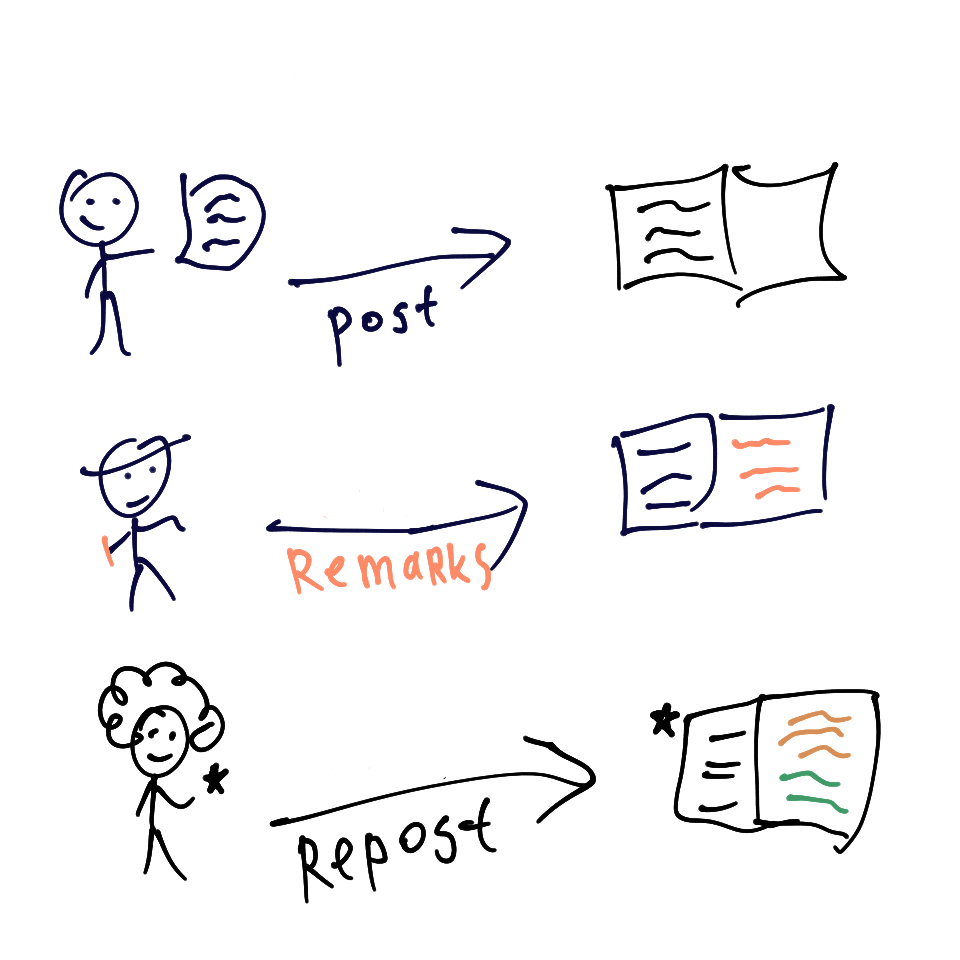
\includegraphics[width=1\textwidth]{fig/users.png}};
    \draw[white,fill] (0,0) rectangle (10,6.4);
  \end{tikzpicture}
\end{frame}

\begin{frame}{}
  \vspace{-3em}
  \begin{tikzpicture}
    \node[anchor=south west,inner sep=0] at (0,0) {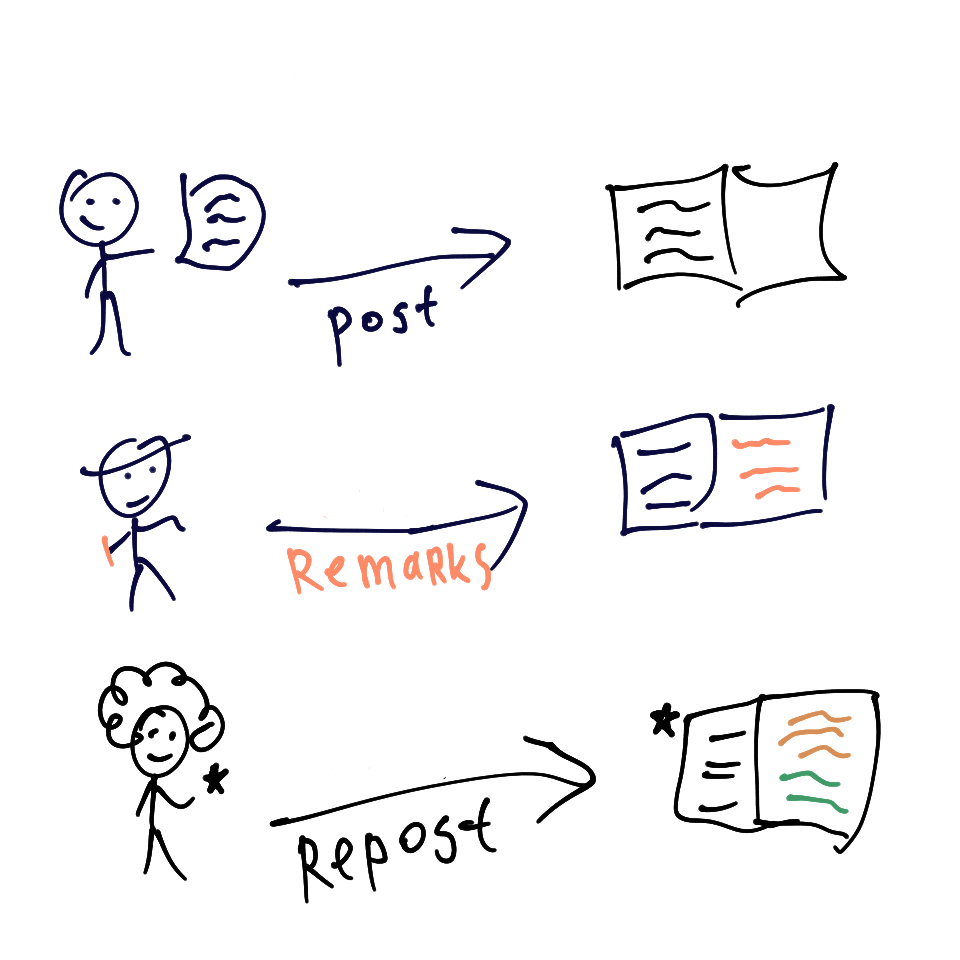
\includegraphics[width=1\textwidth]{fig/users.png}};
    \draw[white,fill] (0,0) rectangle (10,3.8);
  \end{tikzpicture}
\end{frame}

\begin{frame}{}
  \vspace{-3em}
  \begin{tikzpicture}
    \node[anchor=south west,inner sep=0] at (0,0) {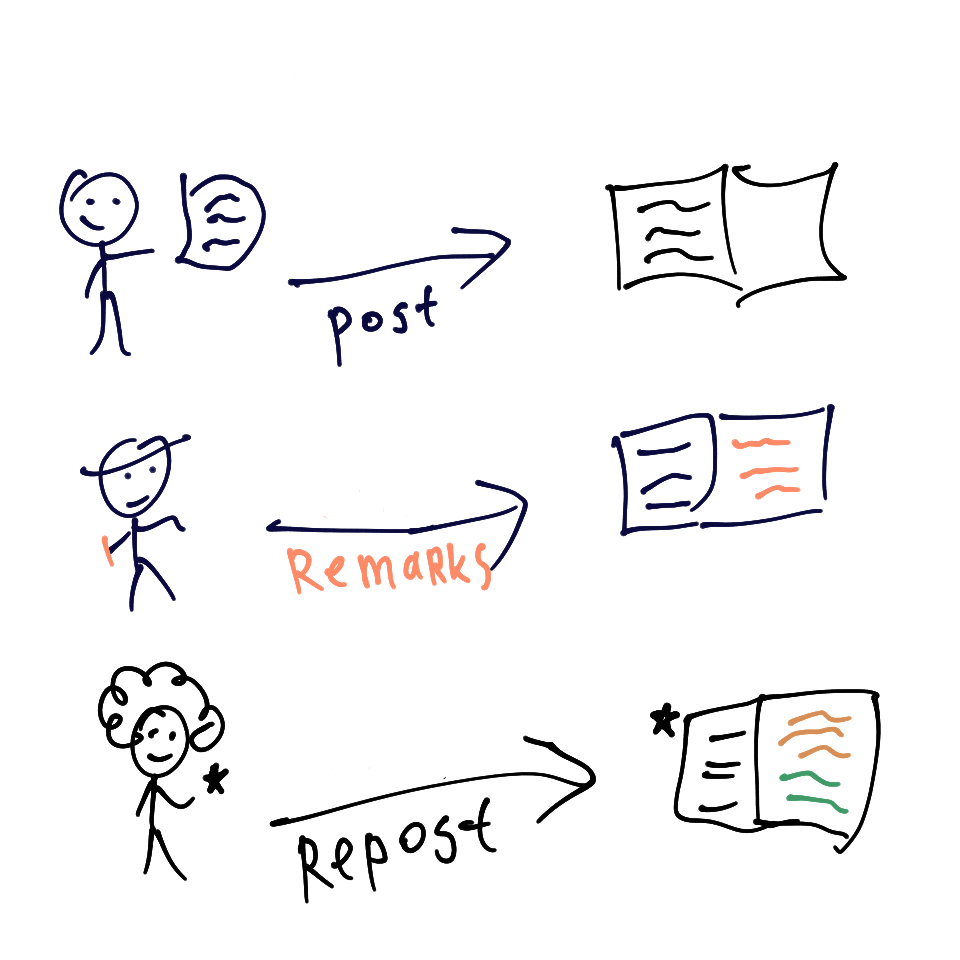
\includegraphics[width=1\textwidth]{fig/users.png}};
    \draw[white,fill] (0,0) rectangle (0,0);
  \end{tikzpicture}
\end{frame}

\begin{frame}{}
  \url{http://papers-gamma.link}
  \vspace{1em}
  
  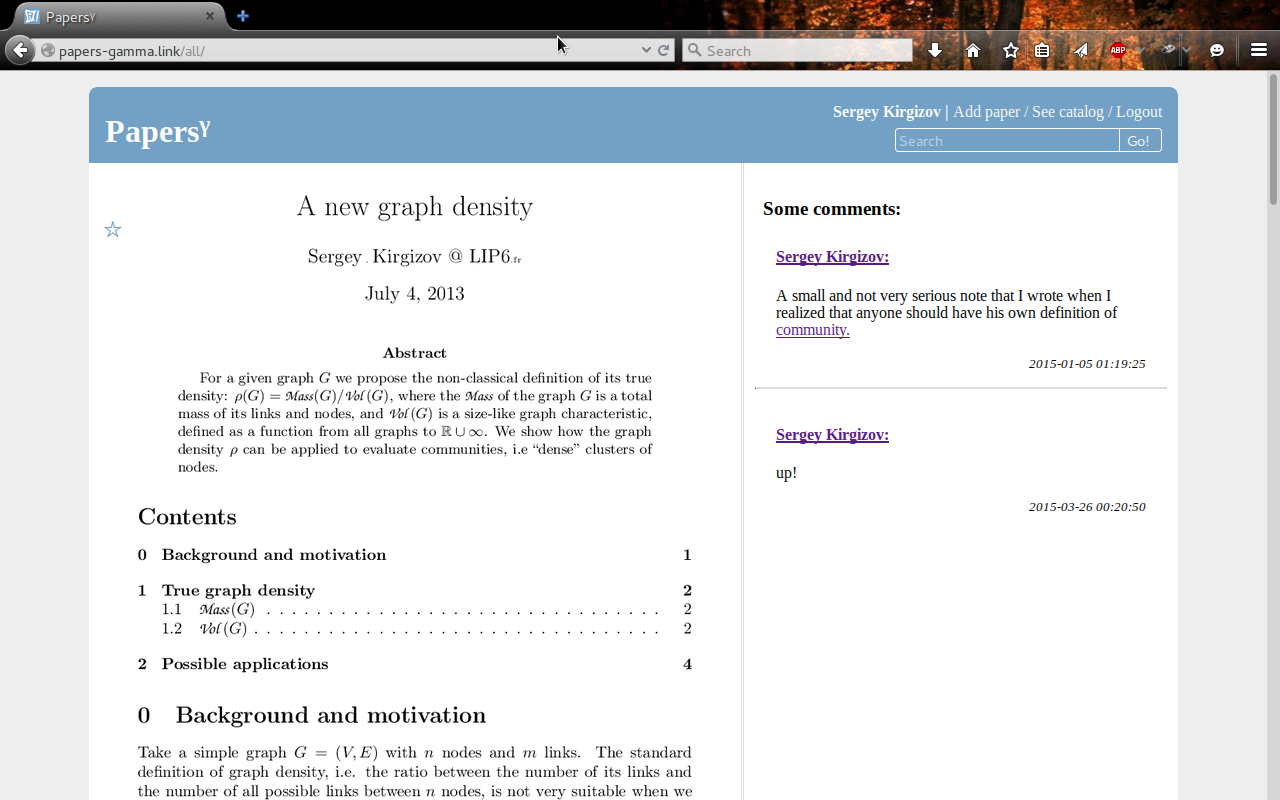
\includegraphics[width=1\textwidth]{fig/papers.png}
  \vspace{2em}

\end{frame}

\begin{frame}{So, what is Papers$^\gamma$ ?}


  $\blacklozenge$ Library of papers/preprints written by you
  \vspace{2em}
  
  $\blacklozenge$  Comfortable place to discuss articles/preprints
  \vspace{2em}
  
  $\blacklozenge$ List of papers/preprints  that you like
  
\end{frame}


\begin{frame}{Simple and ready to hack!}

  \begin{center}
    \setlength\extrarowheight{3pt} 
    
    \begin{tabular}{ l  r }
      \bf & \bf Lines of Code  \\\hline
      HTML+JS & 1000 \\ 
      Python   & 800 \\ 
      CSS      & 520 \\ 
      SQL      & 100 \\ 
      Shell      & 31 \\    \hline
      & \bf2500 
    \end{tabular}
  \end{center}
  
  \scalebox{1.1}{\url{https://github.com/kerzol/papers}}
  \vspace{1em}
  
  \small Local installations can be used as personal or intra-team librarires
  
\end{frame}


\begin{frame}{Thanks to}
  \vfill
  \centering
  
\includegraphics[width=0.28\textwidth]{fig/flask.pdf}
  \hspace{1.7em}
  
\includegraphics[width=0.28\textwidth]{fig/mj_logo.png}
  \hspace{1.7em}
  
\includegraphics[width=0.28\textwidth]{fig/sqlite370_banner.png}

  \vspace{1em}
  
  \Large Marked
  \hspace{1.7em}
  \raisebox{-.3\height}{
\includegraphics[width=0.15\textwidth]{fig/477px-Ghostscript.png}}
  \hspace{1.7em}
  
\includegraphics[width=0.28\textwidth]{fig/559px-JQuery_UI_Logo.png}

\end{frame}





\begin{frame}{TODO}

  $\blacklozenge$ delete/edit papers/comments \\
  $\blacklozenge$ follow, unfollow buttons \\

  \vspace{1em}

  $\blacklozenge$ better search \\
  $\blacklozenge$ private posts \\
  $\blacklozenge$ recommendations \\
  $\blacklozenge$ arxiv/hal/google scholar integration \\

  \vspace{1em}

  ...
  
  \url{https://github.com/kerzol/papers/blob/master/TODO}
  

  
\end{frame}



{
  \mode<all> {
%    \setbeamercolor{background canvas}{bg=structure.fg}
  }
  \begin{frame}[plain]
%    \color{white}
    \vspace{4em}
    \scalebox{1.3}{\Huge Merci beaucoup}
    \vfill
    \hfill
    \scalebox{1.1}{\url{http://papers-gamma.link}}
    %% \vspace{0.7em}
    
    %% \hfill\scalebox{0.9}{\url{https://github.com/kerzol/papers}}
    %% \vspace{0.5em}
    
    %% \hfill\scalebox{0.8}{\url{http://kerzol.github.io/markdown-mathjax}}
    
    
  \end{frame}
}

\end{document}
